\section{Introduction}

Pour mon stage de fin de licence, j'avais un stage de 7 semaines a effectué en entreprise ou en laboratoire en fonction de si l'on voulais s'insérer dans le monde professionnel ou académique. Pour ma part, car je souhaite  m'orienter vers un parcours professionnel, j'ai choisi de faire mon stage en entreprise à Orano.
\subsection{Orano}
Orano est un grand group français spécialisé dans le nucléaire. Elle possède 17 500 collaborateur dans 17 pays et avait un revenu de 4.8 M en 2023\cite{report:rapport_activiter}. Elle est née en 2018 à la suite d'une restructuration d'Areva. Elle est présente dans plusieurs domaines du nucléaire, de l'extraction de l'uranium à la gestion des déchets nucléaires en passant par la production de combustible nucléaire. Ses différentes activité sont répartie dans plusieurs filiales~:
\begin{description}
\item [Orano Support] qui regroupe les activités de support du groupe
\item [Orano Mining] qui regroupe les activités d'extraction d'uranium
\item [Orano Medical] qui regroupe les activités de production de radioéléments pour la médecine nucléaire
\item [Orano Batteries] qui regroupe les activités de recyclage de batterie
\item [Orano Dismantling] qui regroupe les activités de démantèlement de centrale nucléaire
\item [Orano Chimie-Enrichissement] qui regroupe les activités de chimie et d'enrichissement de l'uranium
\end{description}
\begin{figure}
    \centering
    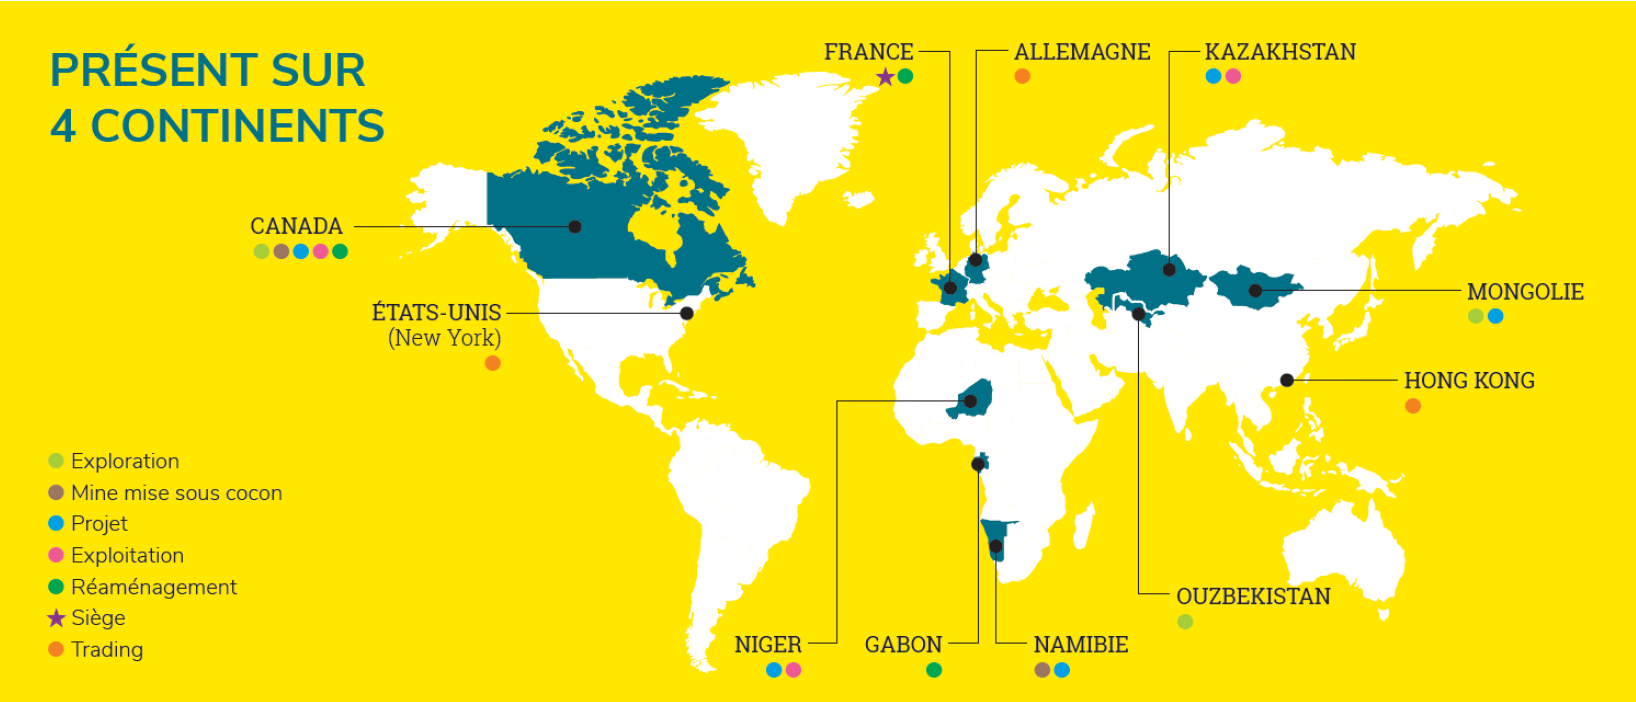
\includegraphics[width=0.5\textwidth]{img/Carte-ornao-international.png}
    \caption[Carte des activités d’Orano dans le monde]{Carte des activités d’Orano dans le monde, Source~:~Dossier d’information Orano 2020}
    \label{fig_carte_orano}
\end{figure}









Ces filiales sont présente a l'international avec des mines d'uranium au Kazakhstan, au Canada et au Niger, de l'exploration ou des projet en Namibie, en Ouzbékistan et en Mongolie. La majorité des sites a l'étranger d'Orano sont des site d'Orano Mining due a la nature de ses activités. C'est dans cette dernière que j'ai effectuée mon stage.
\subsection{Orano Mining}

Orano mining est en charge de tout ce qui est relatif a l'extraction de l'uranium. Nous pouvons repartir ses activités en 4 grands domaines~:
\subsubsection{L'exploration}
L'exploration est la première étape de l'extraction de l'uranium. Elle consiste à trouver des gisements d'uranium. Pour cela, Orano Mining utilise des méthodes géophysiques et géochimiques pour trouver des gisements d'uranium. Une fois un gisement trouvé, il faut l'exploiter.

\subsubsection{L'exploitation}
L'exploitation est la deuxième étape de l'extraction de l'uranium. Elle consiste à extraire l'uranium du sol. Pour cela, Orano Mining utilise diverses méthodes d'extraction en fonction de la nature du gisement. On peut citer~:
\begin{description}
\item [L'extraction in situ] qui consiste a injecter de l'acide dans le sol entre deux couche étanche pour dissoudre l'uranium et le remonter à la surface (voir \cref{ssec_insitu}). C'est le cas des mines de Muyunkum et Tortkuduk au Kazakhstan.
\item [L'extraction par jetboring] qui consiste a creuser un trou dans le sol et a injecter de l'eau sous pression pour remonter l'uranium a la surface (voir \cref{ssec_jetbore}). C'est le cas de la mine Cigar Lake au Canada.
\item [L'extraction à ciel ouvert] qui consiste a creuser une fosse pour extraire l'uranium. C'est le cas de la mine de Somaïr au Niger et de Mclean Lake au Canada (production suspendue entre 2008 et 2025 suite à la chute du cours de l'uranium).
\end{description}

\subsubsection{Le traitement}
Le traitement est la dernière étape de l'extraction de l'uranium. Elle consiste à traiter le minerai pour en extraire l'uranium. Pour cela, Orano Mining utilise des méthodes de traitement chimique pour extraire l'uranium du minerai. Généralement, cette étape est faite avec une lixiviation de l'uranium par une solution concentré acidique, alcaline ou de peroxyde pour former ce que l'on appellera du "yellow cake" due a sa couleur et texture (voir \cref{fig_yellow-cake}). Le yellow cake est composer entre 70\% et 90\% d'oxyde d'uranium notamment d'$U_3O_8$ \cite{article:composition-yellow-cake}. Une fois l'uranium extrait, il est envoyé à Orano Chimie-Enrichissement ou a d'autres partenaires pour être enrichi. En effet, l'uranium naturel est composé a 0,7\% d'uranium 235 et a 99,3\% d'uranium 238\cite{}. Pour être utilisé dans un réacteur, il faut que l'uranium 235 soit enrichi entre 3\% a 5\% d'$U_{238}$\cite{article:uranium-concentration}

\begin{figure}
\centering
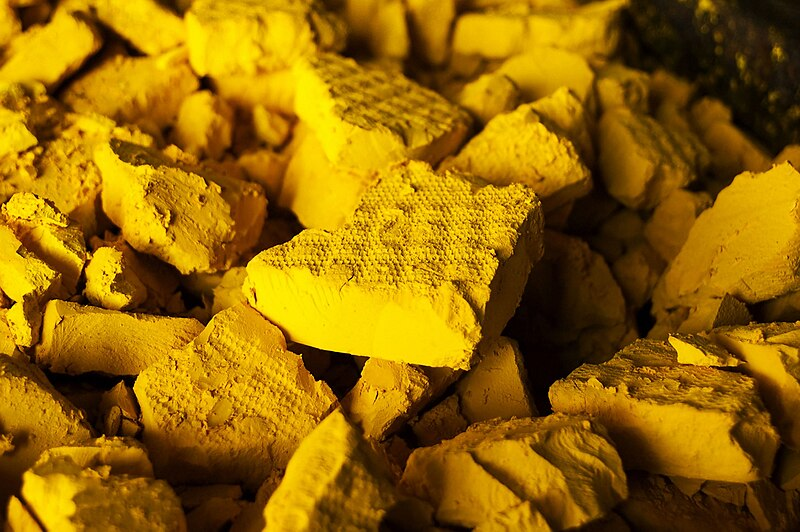
\includegraphics[width=0.5\textwidth]{img/Yellow_Cake_Uranium_(14492248719).jpg}
\caption[Apparence du yellow cake]{Apparence de yellow cake. Avec des méthode modernes, certain traitement preuve lui donner une apparence marron voir noir. Source~:~\href{https://commons.wikimedia.org/wiki/File:Yellow_Cake_Uranium_(14492248719).jpg}{Nuclear Regulatory Commission from US}, Public domain, via Wikimedia Commons}
\label{fig_yellow-cake}
\end{figure}

\subsubsection{L'apres mine}
L'après mine désigne l'ensemble des actions de remédiation et de monitoring qui sont entrepris par Orano après qu'une mine ferme. En effet, une fois une mine fermée, il faut la remettre en état pour éviter les risque de pollution. Pour cela, Orano Mining met en place des système de monitoring pour surveiller l'évolution de la mine et des action de remédiation pour remettre la mine en état. En France, Orano a la charge de 235 sur 247 des site minier d'uranium présent sur le territoire dont des sites qu'Orano n'a pas exploiter \cite{site:orano_apres_mine}. L'après-mine n'intervient pas qu'en France, mais aussi a l'étranger. Par exemple, au Canada, Orano a fini la remédiation de la mine de Cluff Lake (1979-2002) en 2013 et le site a été réouvert au public. En 2023, la gouvernement a été satisfait des actions d'Orano et les terres, on était rendu a l'état provincial \cite{site:Cluff_lake_remediation}.

\subsection{Direction de la transformation digitale}
Au sein de la mine est un petit service qui est en charge de la transformation digitale de la mine. Ce service est en charge de mettre en place divers outils digital pour améliorer les procédures de la mine. Il travaille en collaboration avec les différents services de la mine pour comprendre leur besoin et mettre en place des outils qui répondent a leur besoin. Par exemple un des grand sujet quand j'etais la etait la digitalisation des procedure de Katco, la joint-venure d'Orano au Kazakhstan. Un autre exemple est la documentation; Les différents service produise une quantiter farmineuse de document et de rapport qui ne sont que tres peu utils sous leur format papier. Pour les vieux document il a donc fallut les scanner et il faut indexer tout les document pour rendre les information qu'il contienne accesible. De meme les kilometre de plan geologique qui ont etait produit par les geologue lors des exploration avant les année 2000 sont inutilisable dans leur forme actuel.

Nous cherchons egalement a exploiter les donner que l'on recolte de nos divers activiter pour mieux comprendre comment ont pourrais travailler a l'avenir et ou es ce que on est peu efficace.

\subsection{Choix du Stage}
J'envisage plus tard de devenir ingenieur en \href{https://fr.wikipedia.org/wiki/M%C3%A9catronique}{mecatronique} et j'ai donc chercher un stage qui serait en informatique, en electronique, en mecanique ou idealement un mix des trois. Le nucléaire est egalement un sujet qui m'interesse et dont je comprends un certain nombre de chose. J'ai egalement la conviction que nous ne pourrons pas faire face a la catastrophe climatique qui s'annonce sans le nucléaire. J'ai donc postuler chez Orano pour mon stage de fin de licence. 
\subsection{Objectif du stage}

Orano realise souvant des projet pour ameliorer ses activiter mais souvant il n'y a pas le temps pour revenir sur des projet déjà existant due au taille limiter des equipes. J'ai donc était recruter pour essayer d'apporter des opptimisation a un projet existant: La \nameref{sec_CanOp}. Cette outil a été devloper entre 2018 et 2019 et peser environ 7kg. Pour le confore des operateur emmener a utiliser cette outil il faut le reduire de taille.